\documentclass[a4paper,twoside]{scrartcl}

\usepackage{graphicx,color}
\graphicspath{{images/}{../htdocs/images/header/}}

\usepackage{mparhack}

% \usepackage[a4paper]{geometry}
% \geometry{%
% twoside,%
% %height=.7\paperheight,%
% %width=.7\paperwidth,%
% top=.1\paperheight,%
% bottom=.2\paperheight,%
% left=.1\paperwidth,%
% right=.2\paperwidth%
% %bindingoffset
% }

\usepackage{fancyhdr}
\pagestyle{fancy}
\fancyhead{}
\fancyfoot{}
\fancyfoot[LE,RO]{\iffloatpage{}{\thepage}}
\renewcommand{\headrulewidth}{0pt}
\renewcommand{\footrulewidth}{0pt}
\setlength{\oddsidemargin}{.1\paperwidth}
\setlength{\evensidemargin}{.2\paperwidth}
\setlength{\headheight}{.1\paperheight}
\setlength{\headsep}{0pt}
\setlength{\topmargin}{0pt}
\setlength{\voffset}{-1in}
\setlength{\hoffset}{-1in}
\setlength{\textwidth}{.7\paperwidth}
\setlength{\textheight}{.7\paperheight}
\setlength{\marginparwidth}{.1\paperwidth}

\newcommand{\nicesection}[2]{%
\cleardoublepage
\fbox{\includegraphics[width=\linewidth]{#1}}%
\vspace*{-1em}%
\section{\hfill #2}
\hrule
\vspace*{\baselineskip}%
}

\fboxsep0pt
\setlength{\parindent}{0pt}

\newcommand{\todo}[1]{{\color{red}\bf TODO: #1}}
\newcommand{\comment}[1]{}
\definecolor{codecol}{rgb}{0.1,0.2,0.5}
\newcommand{\code}[1]{\texttt{\color{codecol}#1}}

\frenchspacing
% \usepackage[T1]{fontenc}
% \usepackage[condensed,math]{iwona}

%\usepackage[T1]{fontenc}
%\usepackage[urw-garamond]{mathdesign}

\usepackage[T1]{fontenc}
\usepackage[scaled]{helvet}
\renewcommand{\familydefault}{\sfdefault}

%\setkomafont{sectioning}{\sfdefault}


\title{Darktable Programmer's Guide}
\author{hanatos}

\begin{document}

\fbox{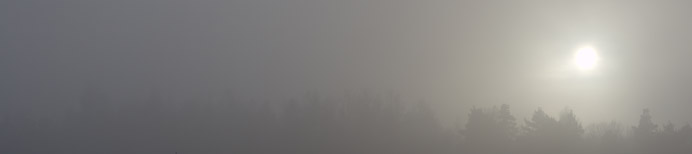
\includegraphics[width=\linewidth]{header12}}%
\vspace*{-1em}%
\section*{\hfill Darktable Programmer's Guide}
\hrule

\vspace*{4\baselineskip}

{\hfill version \input version.tex }

\thispagestyle{empty}

\newpage
\tableofcontents


\nicesection{header1}{Introduction}
\label{sec:introduction}


\nicesection{header2}{System Layout}

\resizebox{\linewidth}{!}{\input{graphs/system.pdftex_t}}

\subsection{Module Descriptions}

\begin{description}
  \item[gui] using gtk2 and cairo.
\end{description}
\begin{description}
  \item[control]
  \item[control, scheduler] using pthreads and a custom job queuing system.
\end{description}
\begin{description}
  \item[image]
  \item[image cache]
  \item[mipmap cache]
  \item[db]
  \item[imageio]
\end{description}
\begin{description}
  \item[library] this is the lighttable module.
  \item[film]
\end{description}
\begin{description}
  \item[develop] this implements the darktable.
  \item[pixelpipe]
  \item[image operation (iop) modules, aka plug-ins]
\end{description}

\subsection{Image Loading Data Flow}

\paragraph{Related Modules}
\begin{itemize}
  \item imageio \code{dt\_imageio\_*}
  \item db (messily hidden in sqlite3 statements all over the place)
  \item image cache \code{dt\_image\_cache\_*}
  \item mip cache \code{dt\_mipmap\_cache\_*}
  \item image \code{dt\_image\_t}
\end{itemize}

\paragraph{in image cache}
\begin{itemize}
  \item \code{dt\_image\_import}

  db $\rightarrow$ image struct, trigger imageio disk $\rightarrow$ image entry in db if miss,
                metadata through libraw/magick
  
 
\end{itemize}

\paragraph{in mip cache}
\begin{itemize}
  \item \code{dt\_image\_get}

      db $\rightarrow$ mip[0--4], trigger imageio disk $\rightarrow$ mip4 and mip4 $\rightarrow$ mip[0-3] if miss.

  
      db $\rightarrow$ mipf, trigger mip4 $\rightarrow$ mipf or pixels $\rightarrow$ mipf if miss.
\end{itemize}

\paragraph{in imageio}
\begin{itemize}
  \item \code{dt\_imageio\_open\_preview}

    disk $\rightarrow$ mip[0--4] entries in db (load thumbnail).
    \begin{itemize}
      \item[\todo{}]  \code{dt\_imageio\_open\_ldr\_preview}
      \item \code{dt\_imageio\_open\_raw\_preview}
    \end{itemize}
  \item mip4 $\rightarrow$ mipf (by guessed reverse gamma) \code{dt\_image\_preview\_to\_raw}.
  \item full pixels $\rightarrow$ mipf (downscaling) \code{dt\_image\_raw\_to\_preview}.
  \item mip4 $\rightarrow$ mip[0--3] \code{dt\_image\_update\_mipmaps}.
\end{itemize}

image import: only load \code{dt\_image\_t} and mip[0--4] to database.

\code{dt\_image\_get}: check mipmap cache, check database, else \code{dt\_imageio\_open[\_preview]}.

\subsection{Cache Interfaces}

\subsubsection{Image Cache}

\code{dt\_image\_cache\_t}

\subsubsection{Mipmap Cache}

\code{dt\_image\_t}

\begin{description}
  \item{\code{dt\_image\_get}} get buffer or, if missed, a lower resolution (launch job in bg for correct resolution)
  \item{\code{dt\_image\_load}} Load buffer in this thread, return exactly this resolution.
    No locking is performed, so be sure to acquire the lock using \code{dt\_image\_alloc} before.
\end{description}

\subsubsection{Homebrew Pixelpipe Cache}

\subsection{Plug-in Interface}

For examples, have a look at \code{src/iop/*.\{h,c\}}.

\subsubsection{Gui Callbacks}

\subsubsection{Image Processing}

State of libgegl support: enable at compile time with \texttt{--enable-gegl}. Using this
flag is discouraged at the moment, as libgegl is really a lot slower than the homebrew version.

\end{document}
